%%%%%%%%%%%%%%%%%%%%%%%%%%%%%%%%%%%%%%%%%%%%%%%%%%%%%%%%%%%%%%%%%%%%%
%% This is a (brief) model paper using the achemso class
%% The document class accepts keyval options, which should include
%% the target journal and optionally the manuscript type. 
%%%%%%%%%%%%%%%%%%%%%%%%%%%%%%%%%%%%%%%%%%%%%%%%%%%%%%%%%%%%%%%%%%%%%
\documentclass[journal=jacsat,manuscript=article]{achemso}
\usepackage{subcaption}
\usepackage{graphicx}
\usepackage{array}
\usepackage{adjustbox}
\usepackage{longtable}
\usepackage{xcolor}
\usepackage[normalem]{ulem} 
%%%%%%%%%%%%%%%%%%%%%%%%%%%%%%%%%%%%%%%%%%%%%%%%%%%%%%%%%%%%%%%%%%%%%
%% Place any additional packages needed here.  Only include packages
%% which are essential, to avoid problems later. Do NOT use any
%% packages which require e-TeX (for example etoolbox): the e-TeX
%% extensions are not currently available on the ACS conversion
%% servers.
%%%%%%%%%%%%%%%%%%%%%%%%%%%%%%%%%%%%%%%%%%%%%%%%%%%%%%%%%%%%%%%%%%%%%
\usepackage[version=3]{mhchem} % Formula subscripts using \ce{}

%%%%%%%%%%%%%%%%%%%%%%%%%%%%%%%%%%%%%%%%%%%%%%%%%%%%%%%%%%%%%%%%%%%%%
%% If issues arise when submitting your manuscript, you may want to
%% un-comment the next line.  This provides information on the
%% version of every file you have used.
%%%%%%%%%%%%%%%%%%%%%%%%%%%%%%%%%%%%%%%%%%%%%%%%%%%%%%%%%%%%%%%%%%%%%
%%\listfiles

%%%%%%%%%%%%%%%%%%%%%%%%%%%%%%%%%%%%%%%%%%%%%%%%%%%%%%%%%%%%%%%%%%%%%
%% Place any additional macros here.  Please use \newcommand* where
%% possible, and avoid layout-changing macros (which are not used
%% when typesetting).
%%%%%%%%%%%%%%%%%%%%%%%%%%%%%%%%%%%%%%%%%%%%%%%%%%%%%%%%%%%%%%%%%%%%%
\newcommand*\mycommand[1]{\texttt{\emph{#1}}}

%%%%%%%%%%%%%%%%%%%%%%%%%%%%%%%%%%%%%%%%%%%%%%%%%%%%%%%%%%%%%%%%%%%%%
%% Meta-data block
%% ---------------
%% Each author should be given as a separate \author command.
%%
%% Corresponding authors should have an e-mail given after the author
%% name as an \email command. Phone and fax numbers can be given
%% using \phone and \fax, respectively; this information is optional.
%%
%% The affiliation of authors is given after the authors; each
%% \affiliation command applies to all preceding authors not already
%% assigned an affiliation.
%%
%% The affiliation takes an option argument for the short name.  This
%% will typically be something like "University of Somewhere".
%%
%% The \altaffiliation macro should be used for new address, etc.
%% On the other hand, \alsoaffiliation is used on a per author basis
%% when authors are associated with multiple institutions.
%%%%%%%%%%%%%%%%%%%%%%%%%%%%%%%%%%%%%%%%%%%%%%%%%%%%%%%%%%%%%%%%%%%%%
\author{Juan Rafael Gomez Quispe}
\affiliation[Universidade Federal do ABC]
{Center of Natural and Human Sciences, Federal University of ABC, Santo Andre, Sao Paulo, Brazil}

\author{Carlos Raul Primo Sapillado}
\affiliation[National University of San Marcos]
{Facultad de Ciencias Físicas, Universidad Nacional Mayor de San Marcos, 15081 Lima, Peru}

\author{Caique C. Oliveira}
\affiliation[Universidade Federal do ABC]
{Center of Natural and Human Sciences, Federal University of ABC, Santo Andre, Sao Paulo, Brazil}

\author{Chachi Rojas-Ayala}
\affiliation[National University of San Marcos]
{Facultad de Ciencias Físicas, Universidad Nacional Mayor de San Marcos, 15081 Lima, Peru}

\author{Pedro Alves da Silva Autreto}
\affiliation[Universidade Federal do ABC]
{Center of Natural and Human Sciences, Federal University of ABC, Santo Andre, Sao Paulo, Brazil}

\email{pedro.autreto@ufabc.edu.br}
\phone{+55 (19) 98279-4988}

\title[An \textsf{achemso} demo]
{Selective HER Activation of Monolayer CrCl$_3$ by Transition-Metal Functionalization}
\abbreviations{CrCl$_{3}$, DFT, MD, HER}
\keywords{CrCl$_{3}$, Density Functional Theory, Molecular Dynamics, Hydrogen Evolution Reaction}

\begin{document}
\begin{suppinfo}

    \begin{figure}[H]
        \centering
        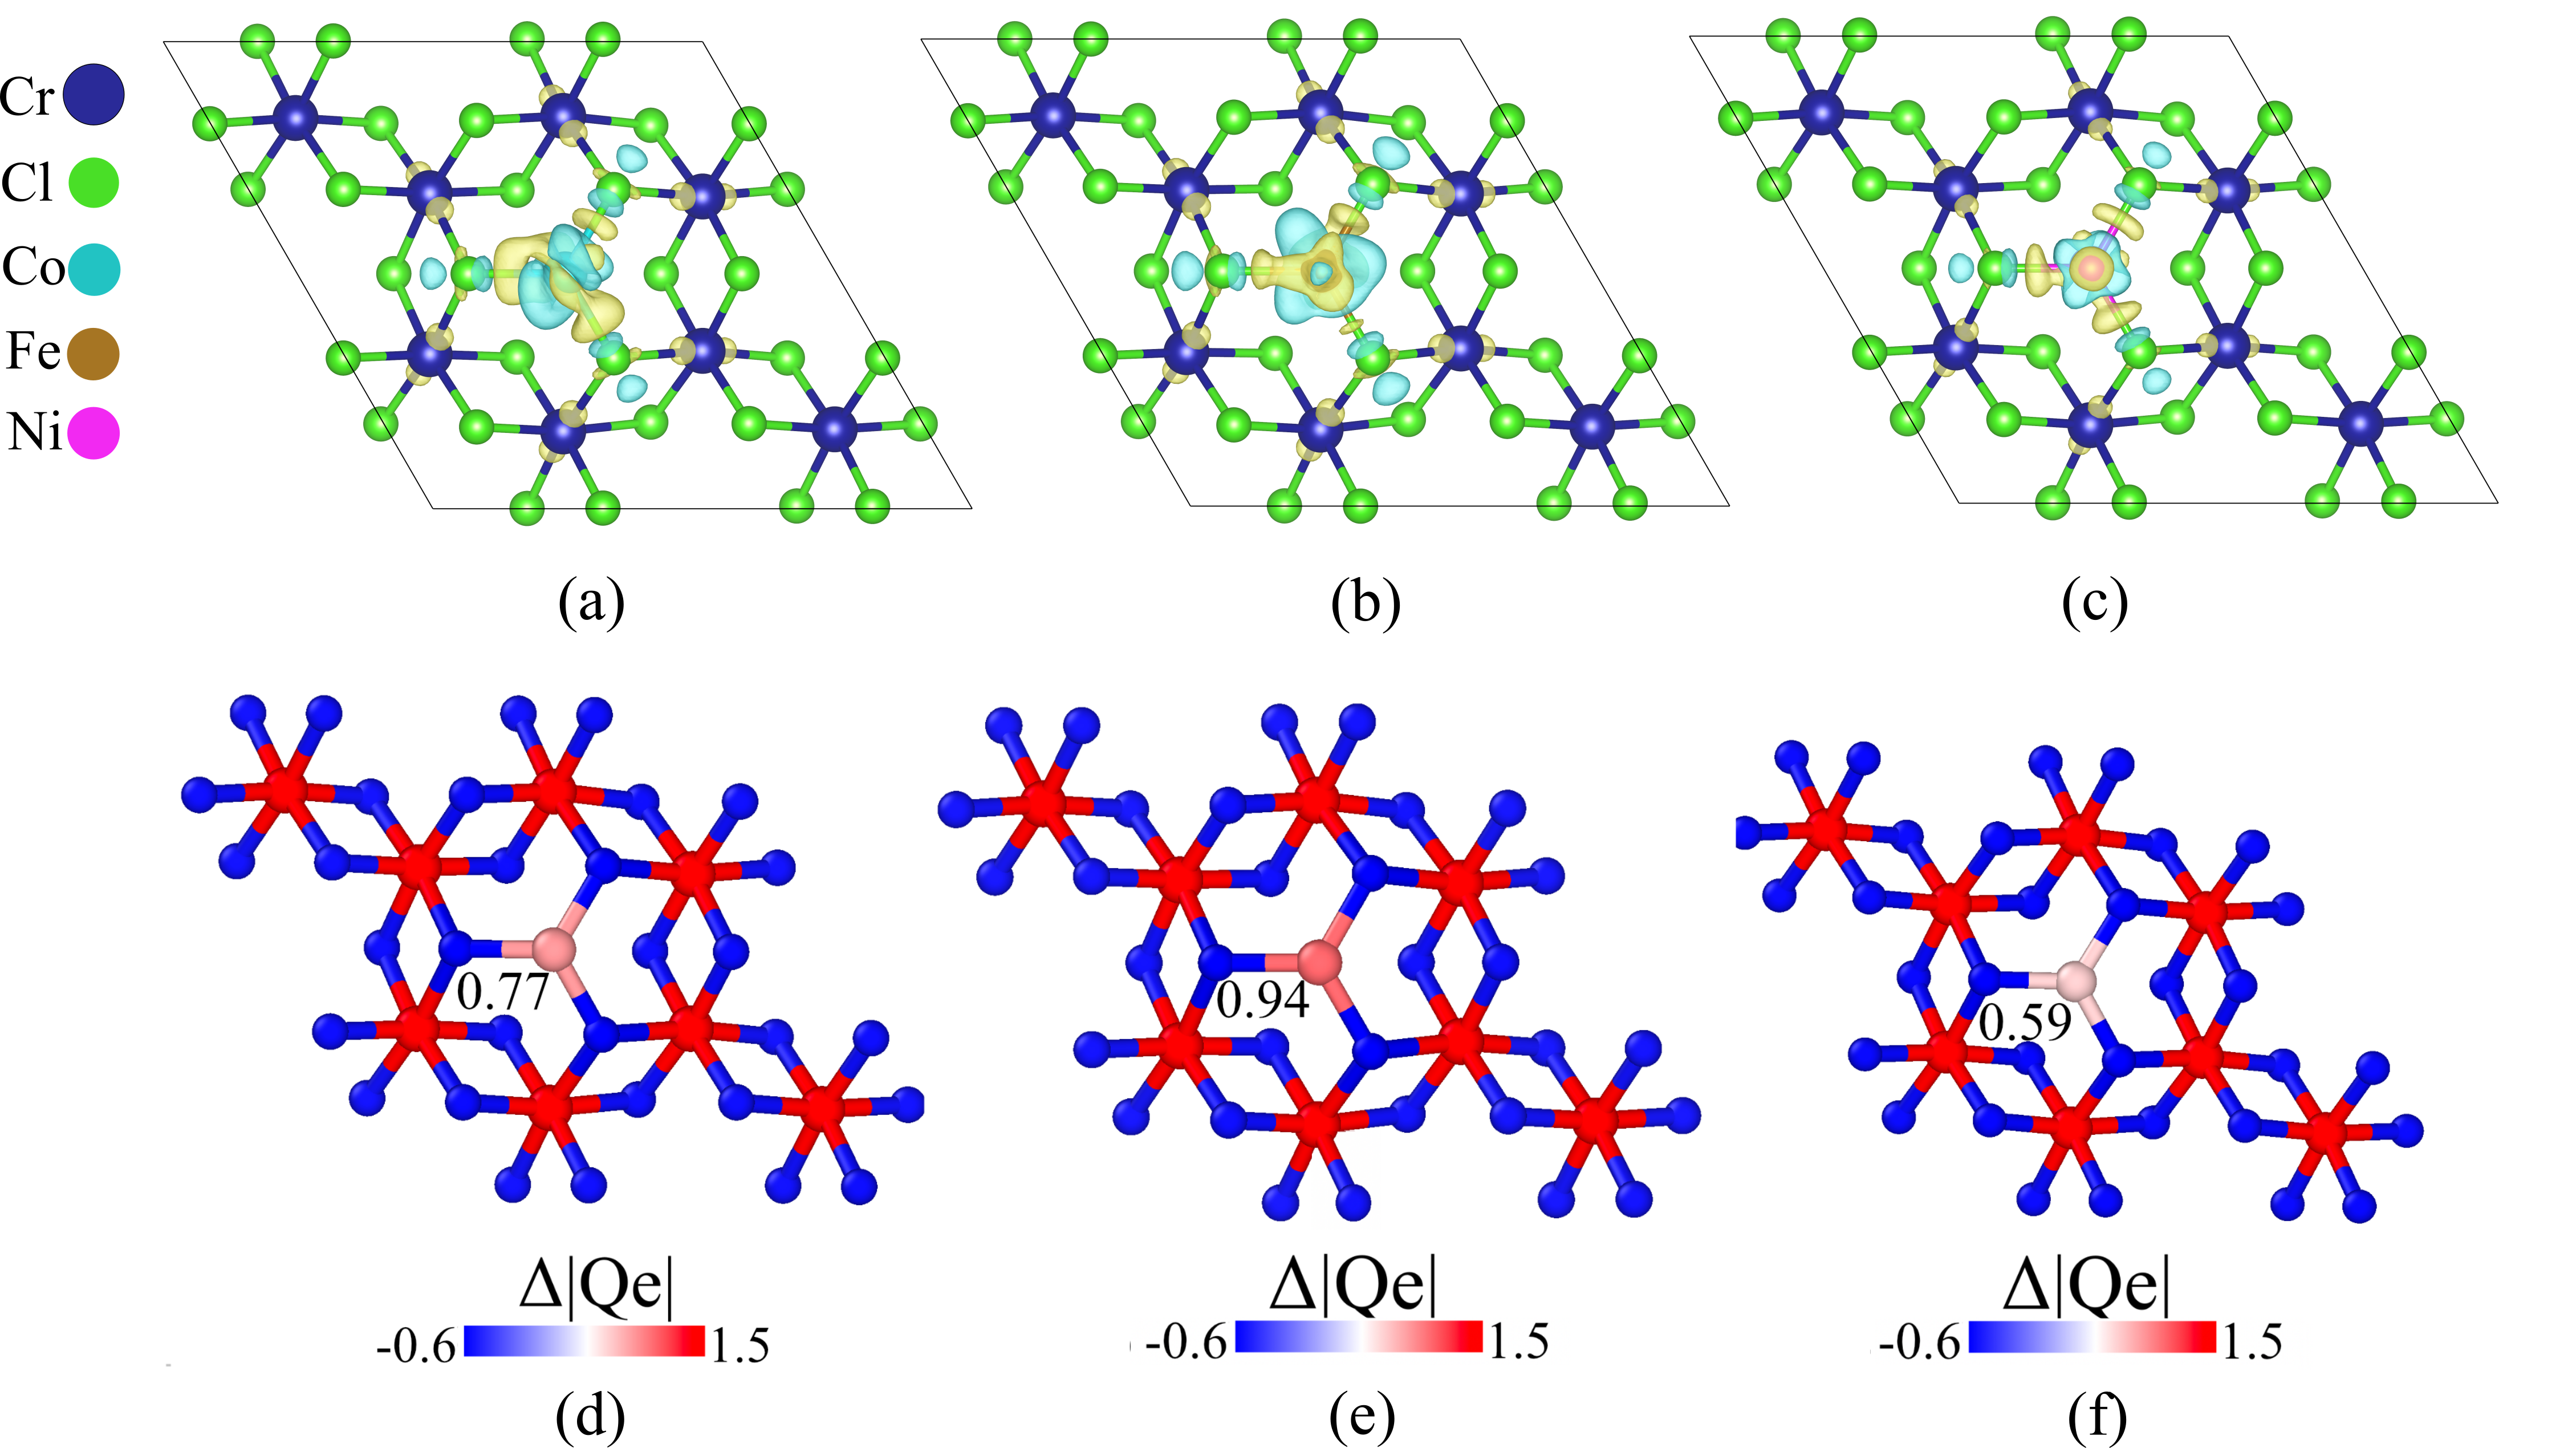
\includegraphics[width=0.9\linewidth]{figure/Fig_SI_1.png}
        \caption*{Fig. S1. Top views of the charge-density-difference isosurfaces for (a) Co-, (b) Fe-, and (c) Ni-adsorbed CrCl$_3$, respectively, plotted at an isosurface value of $\delta = 5^{-3}$ eV/Ang$^{3}$. The two colors denote regions of charge accumulation and charge depletion induced by adatom adsorption. (d-f) Top views of the corresponding Bader charge analysis for Co-, Fe-, and Ni-adsorbed CrCl$_3$, respectively. The values indicated in each panel represent the magnitude of the charge transfer associated with the adsorbed transition-metal atom, in units of $|e|$.}
        \label{fig:S1}
    \end{figure}

    \begin{figure}[H]
        \centering
        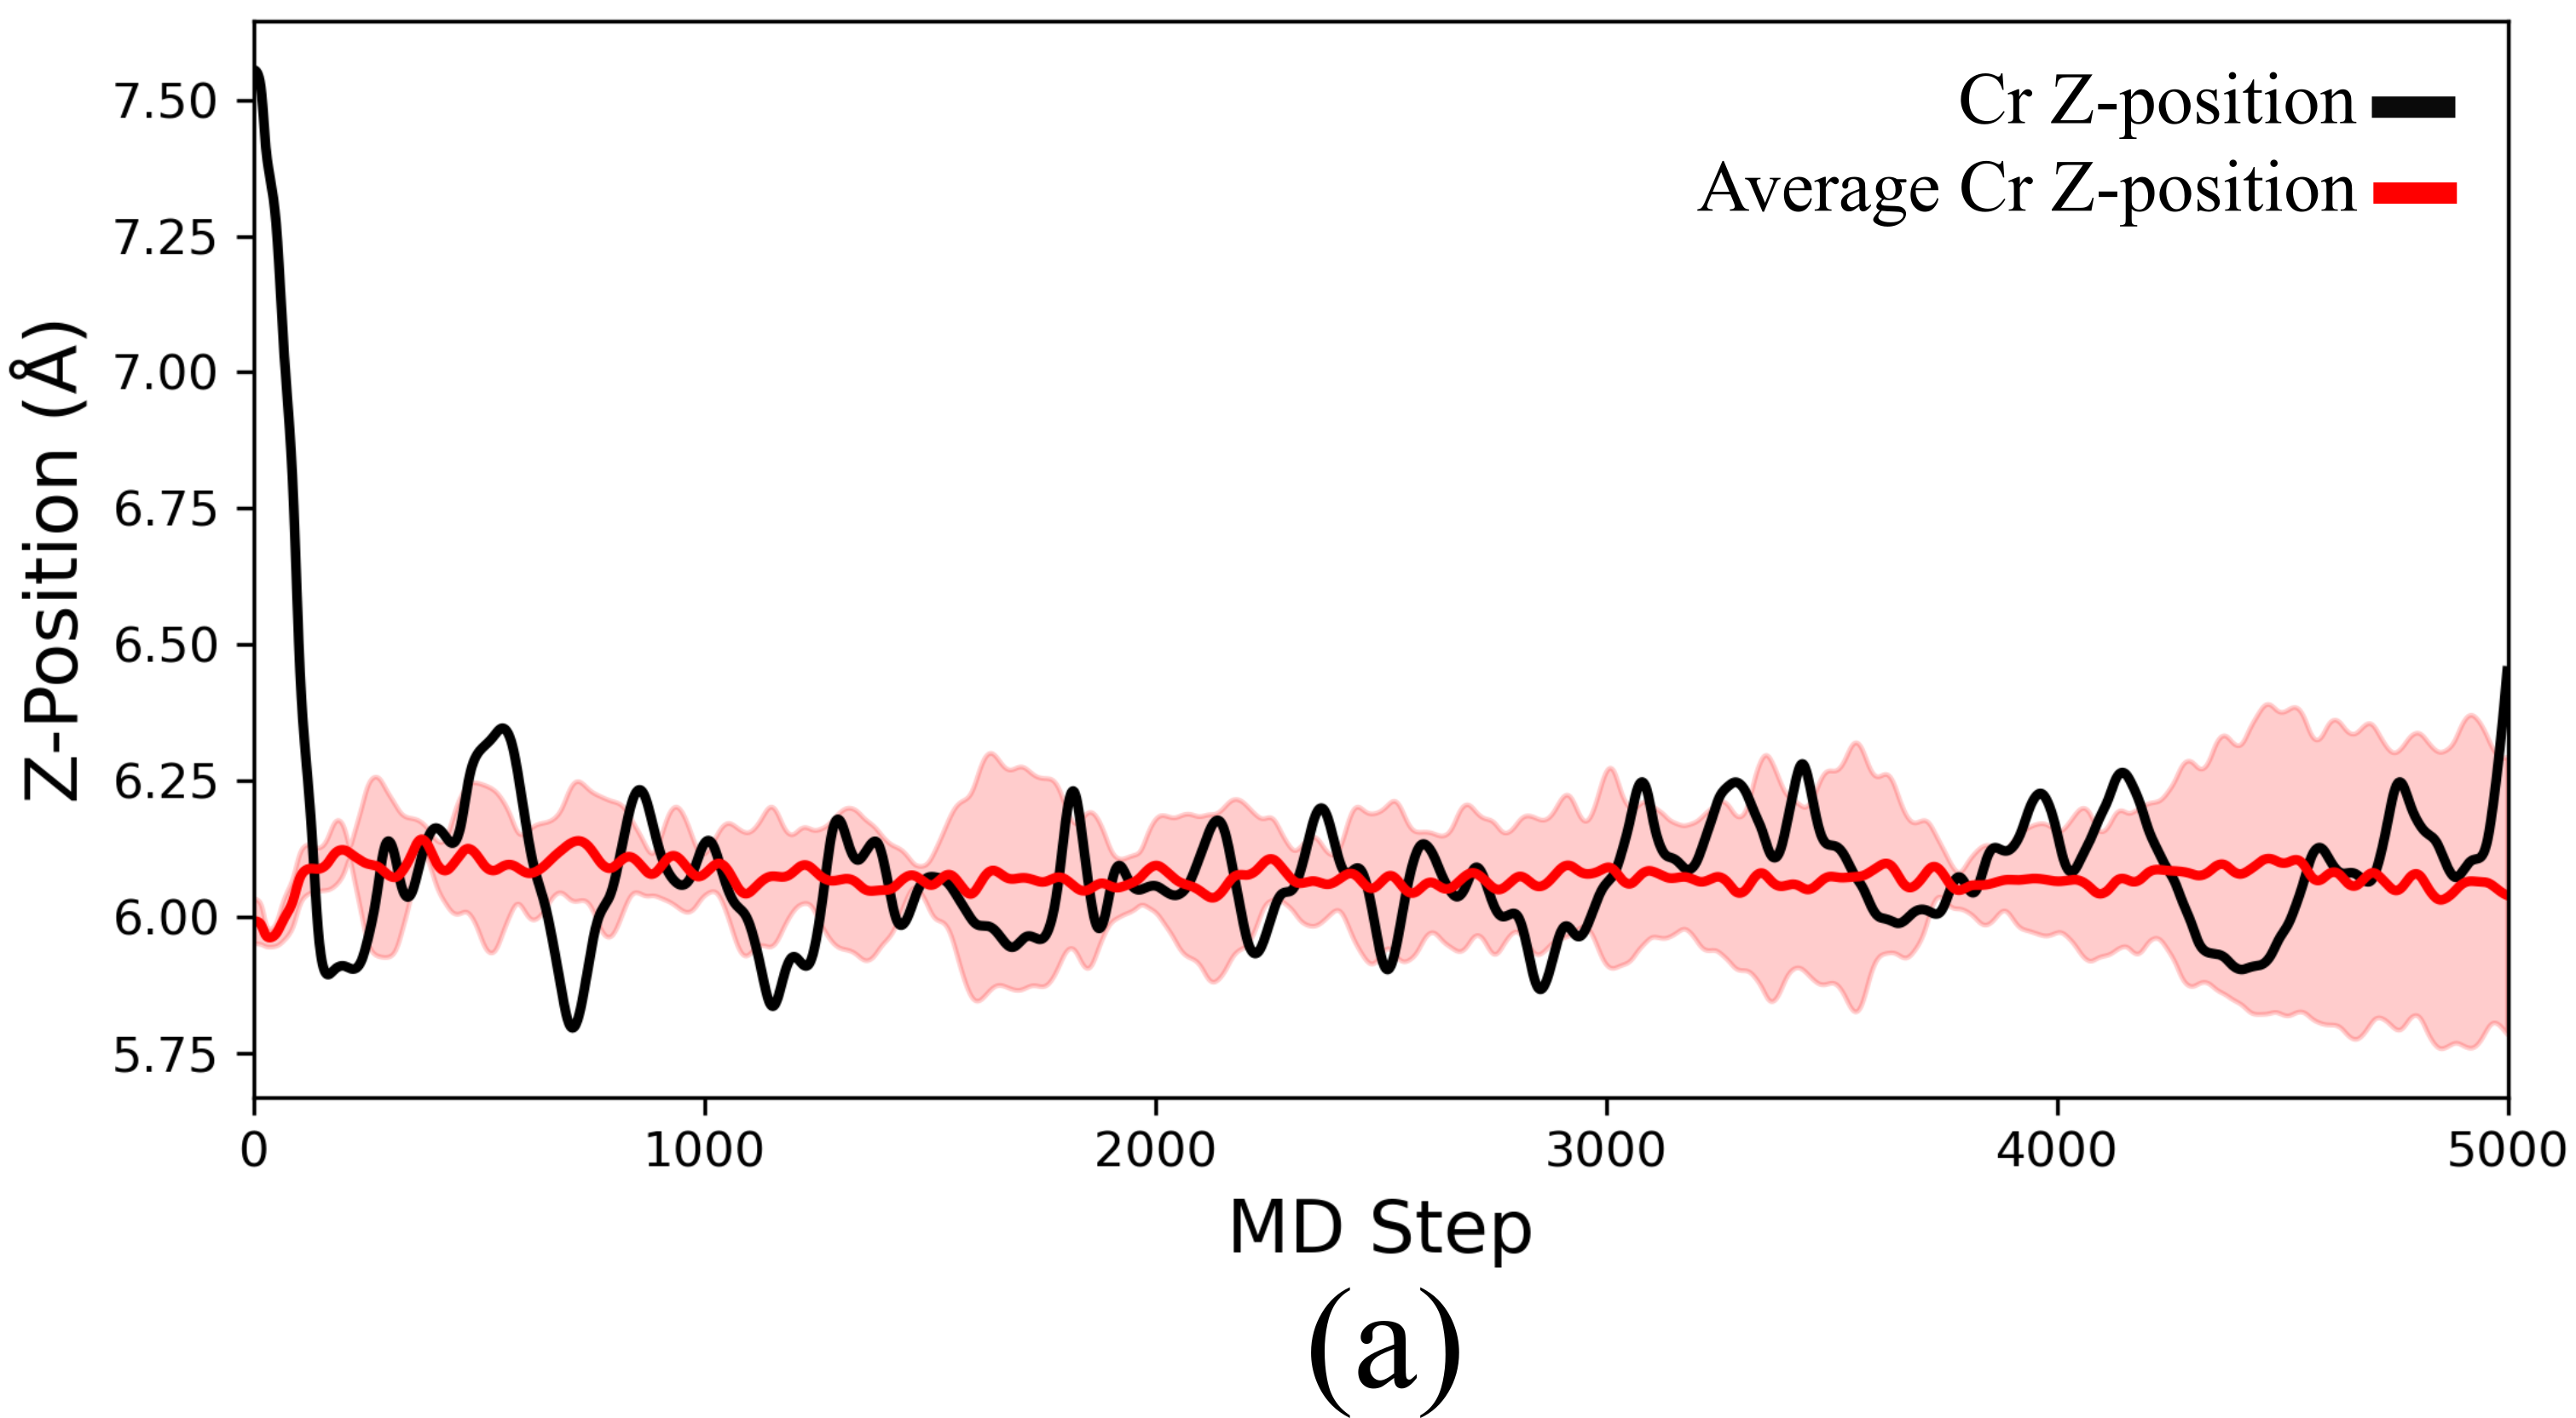
\includegraphics[width=1.0\linewidth]{figure/Fig_SI_2.png}
        \caption*{Fig. S2. Time evolution of the total energy (blue curves, left axis) and instantaneous temperature (red curves, right axis) obtained from the AIMD simulations performed at 300 K for the CrCl$_3$ monolayer with Cr adsorbed at the hollow site.}
        \label{fig:S2}
    \end{figure}

    \begin{figure}[H]
        \centering
        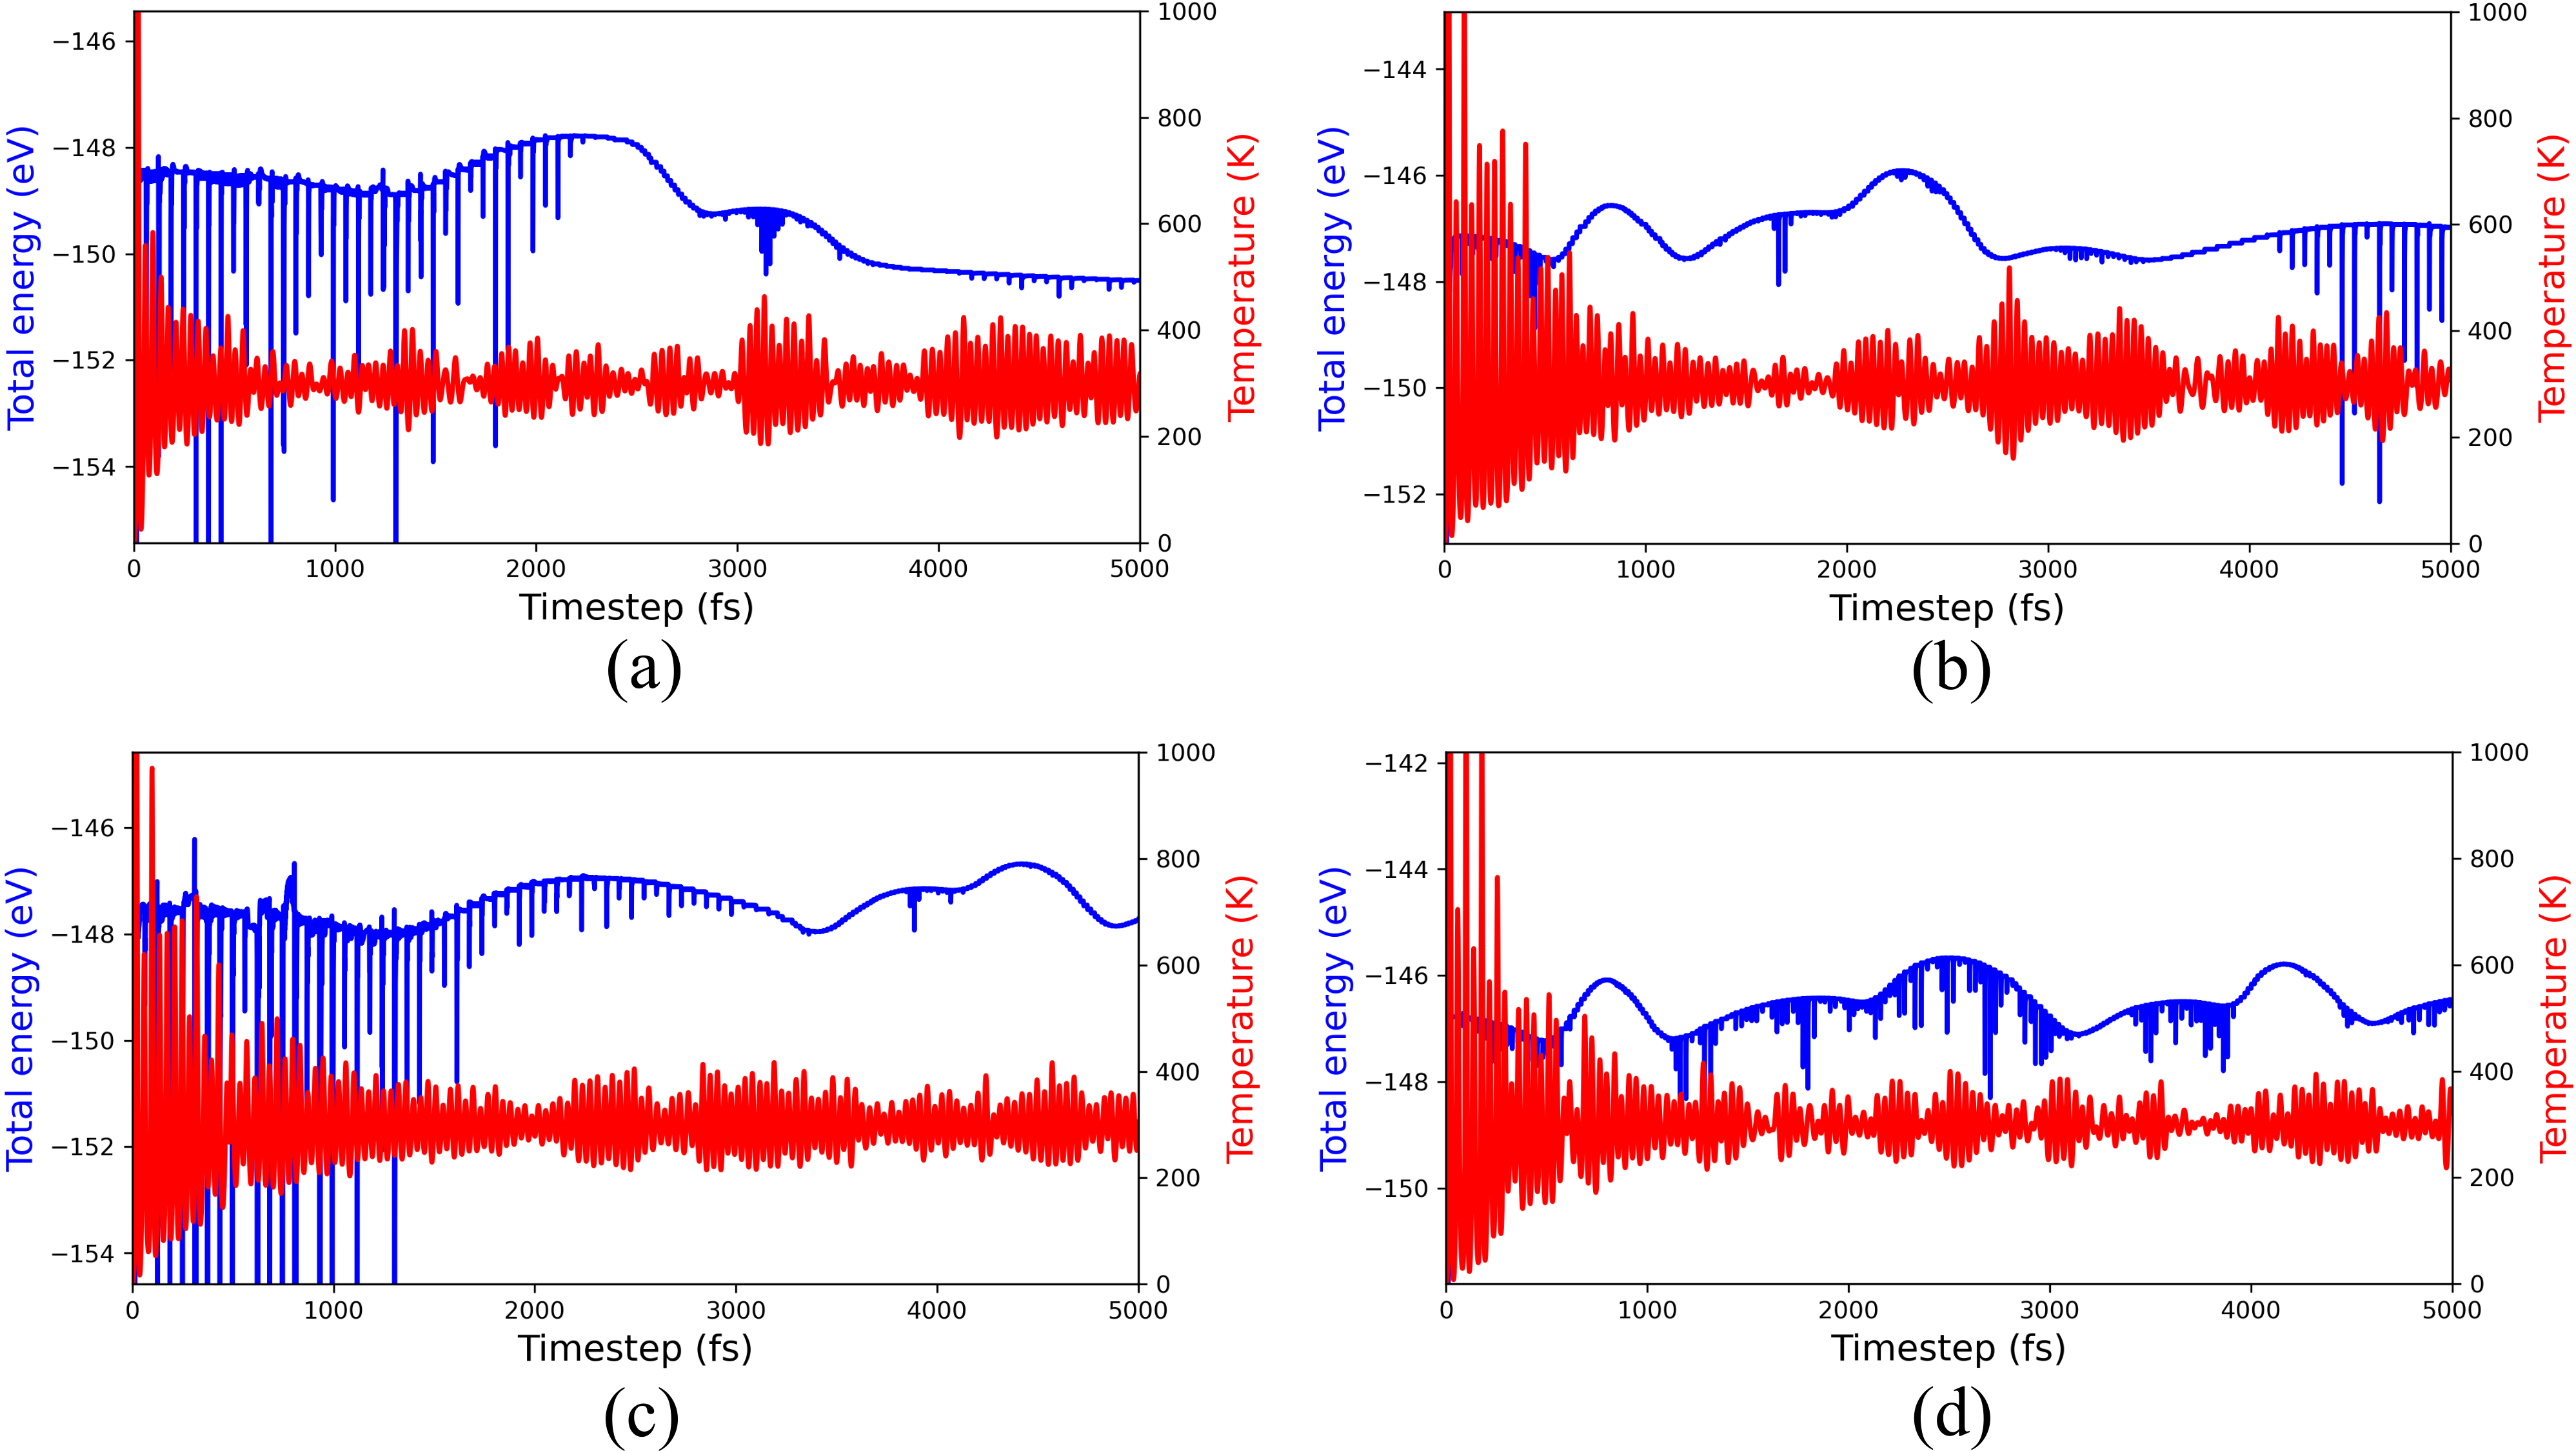
\includegraphics[width=1.0\linewidth]{figure/Fig_SI_3.png}
        \caption*{Fig. S3. Time evolution of the total energy (blue curves, left axis) and instantaneous temperature (red curves, right axis) obtained from the AIMD simulations performed at 300 K for the CrCl$_3$ monolayer with adsorbed (a) Cr, (b) Co, (c) Fe, and (d) Ni atoms at the hollow site. The results confirm the thermal equilibration of all systems during the 5 ps simulation window.}
        \label{fig:S3}
    \end{figure}

    \begin{figure}[H]
        \centering
        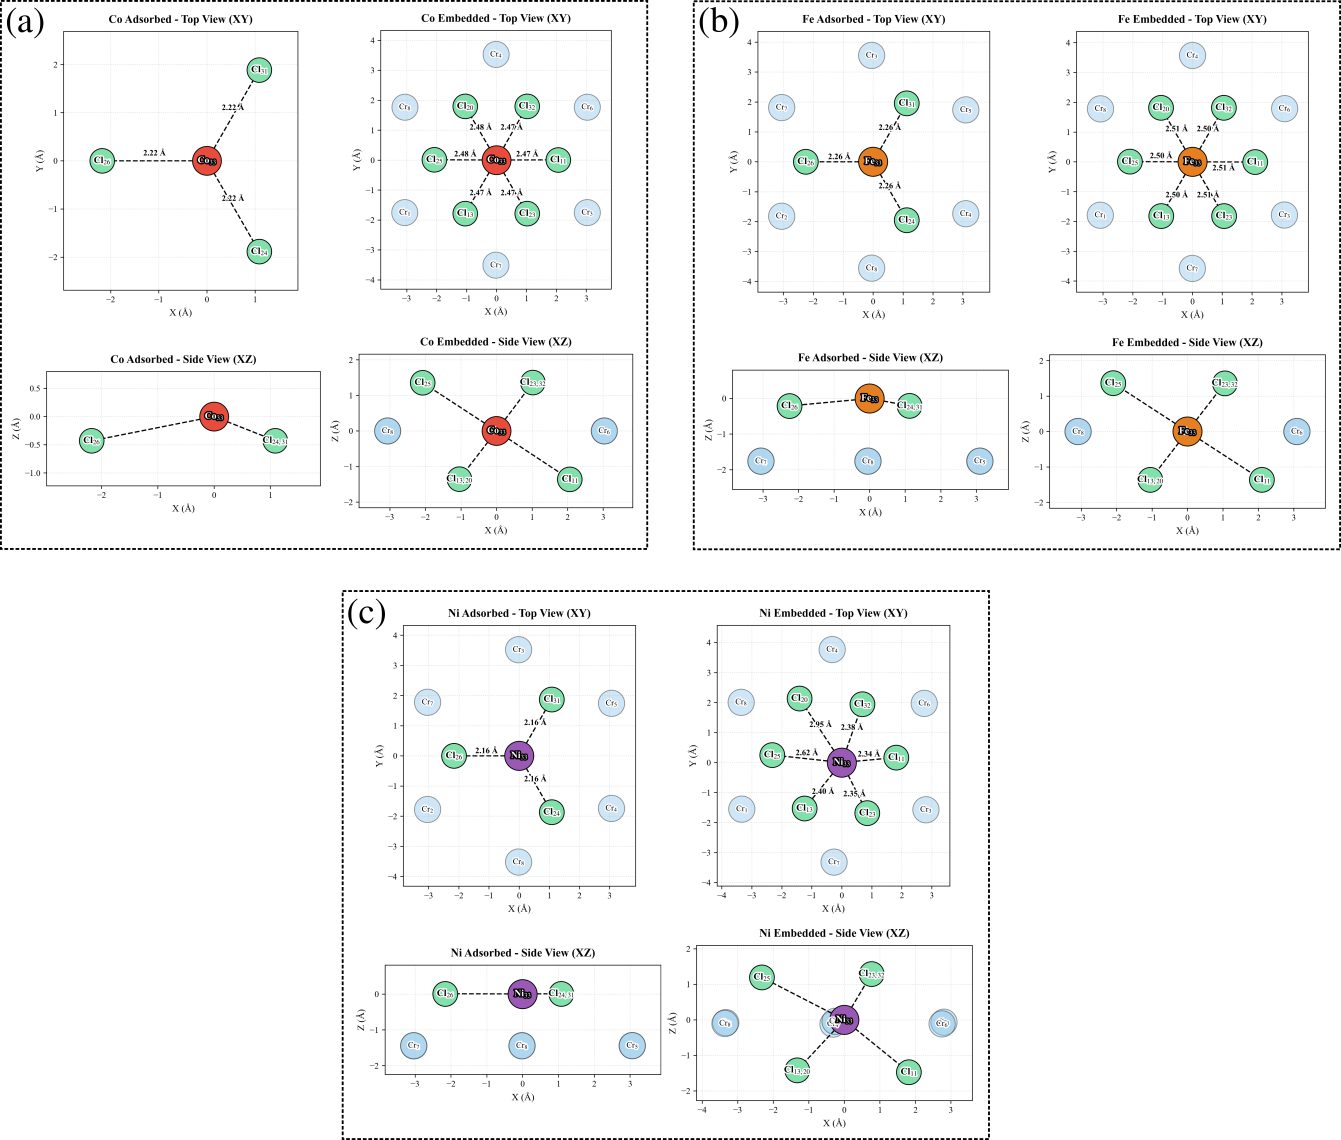
\includegraphics[width=1.0\linewidth]{figure/new_sup_fig_1.png}
        \caption*{Fig. S4. Schematic top ($XY$) and side ($XZ$) views of the optimized local coordination geometries and TM--Cl bond lengths (\AA) for (a) Co-, (b) Fe-, and (c) Ni-functionalized monolayer CrCl$_3$ in both adsorbed (hollow site, 3-fold coordinated) and embedded (6-fold octahedrally coordinated) configurations. Light blue, light green, and red/orange/purple spheres represent Cr, Cl, and transition-metal (Co, Fe, Ni) atoms, respectively.}
        \label{fig:S4}
    \end{figure}

    \begin{figure}[H]
        \centering
        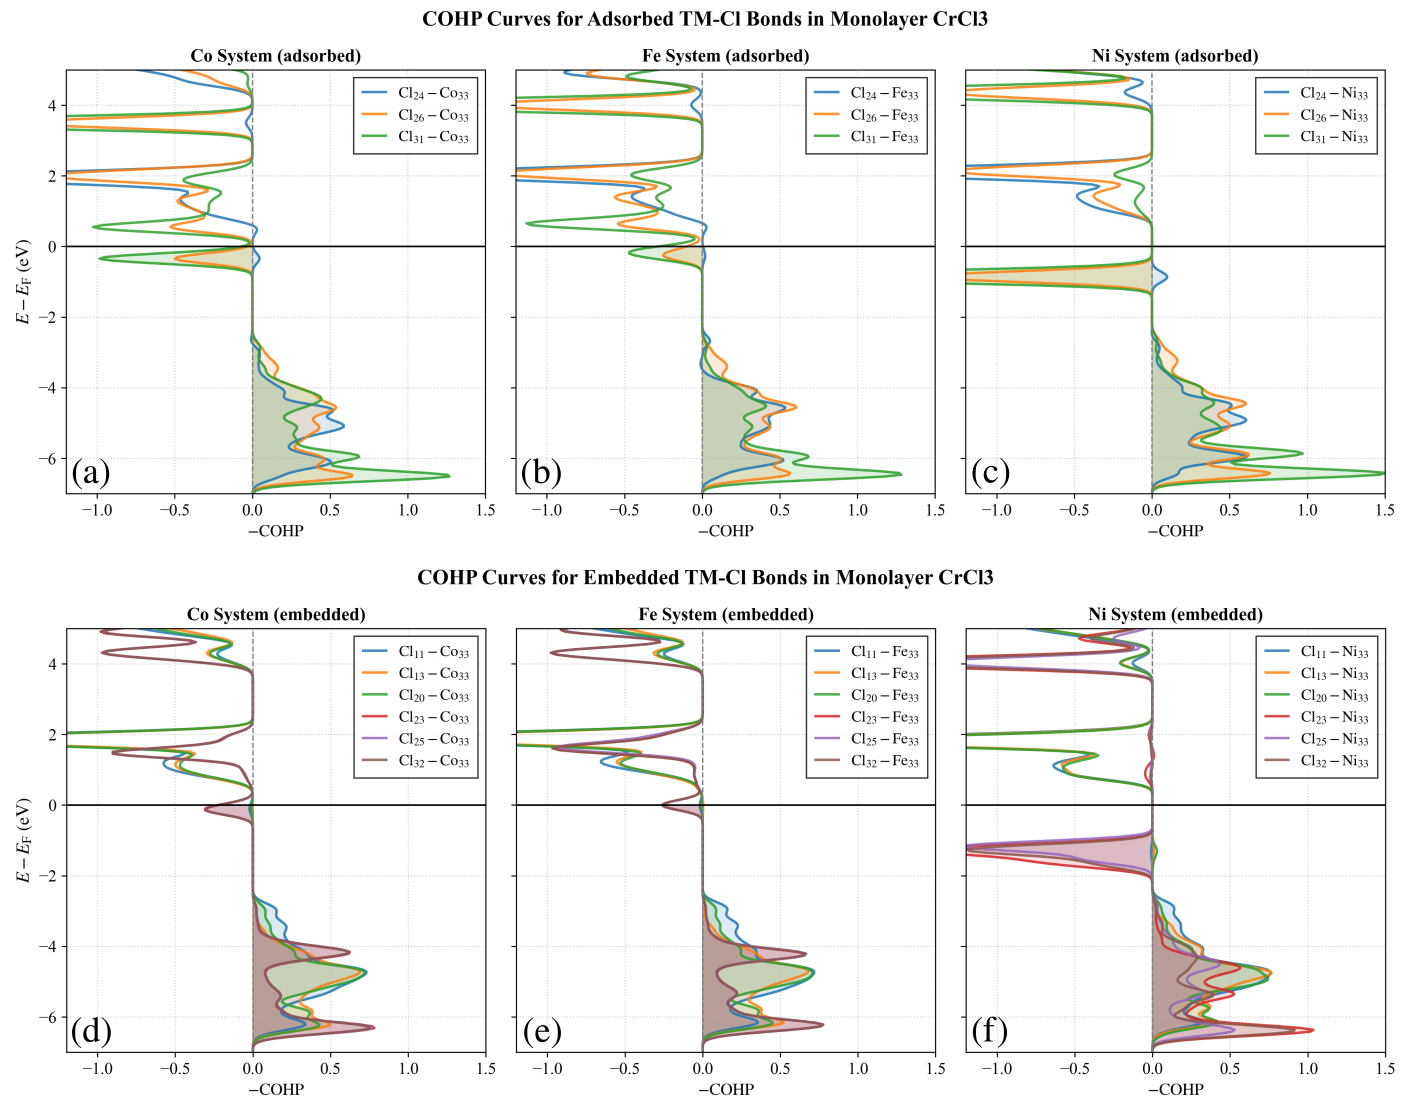
\includegraphics[width=1.0\linewidth]{figure/new_sup_fig_2.png}
        \caption*{Fig. S5. Crystal Orbital Hamilton Population ($-\mathrm{COHP}$) energy curves calculated for the individual TM--Cl (TM = Co, Fe, Ni) chemical bonds in monolayer CrCl$_3$. (a--c) $-\mathrm{COHP}$ diagrams for the 3-fold coordinated adsorbed Co, Fe, and Ni systems, respectively. (d--f) $-\mathrm{COHP}$ diagrams for the 6-fold octahedrally coordinated embedded Co, Fe, and Ni systems, respectively. The horizontal black line indicates the Fermi level ($E - E_{\mathrm{F}} = 0$ eV). Shaded regions below $E_{\mathrm{F}}$ highlight bonding orbital contributions ($-\mathrm{COHP} > 0$), while curves extending into negative values denote anti-bonding states.}
        \label{fig:S5}
    \end{figure}

    \begin{figure}[H]
        \centering
        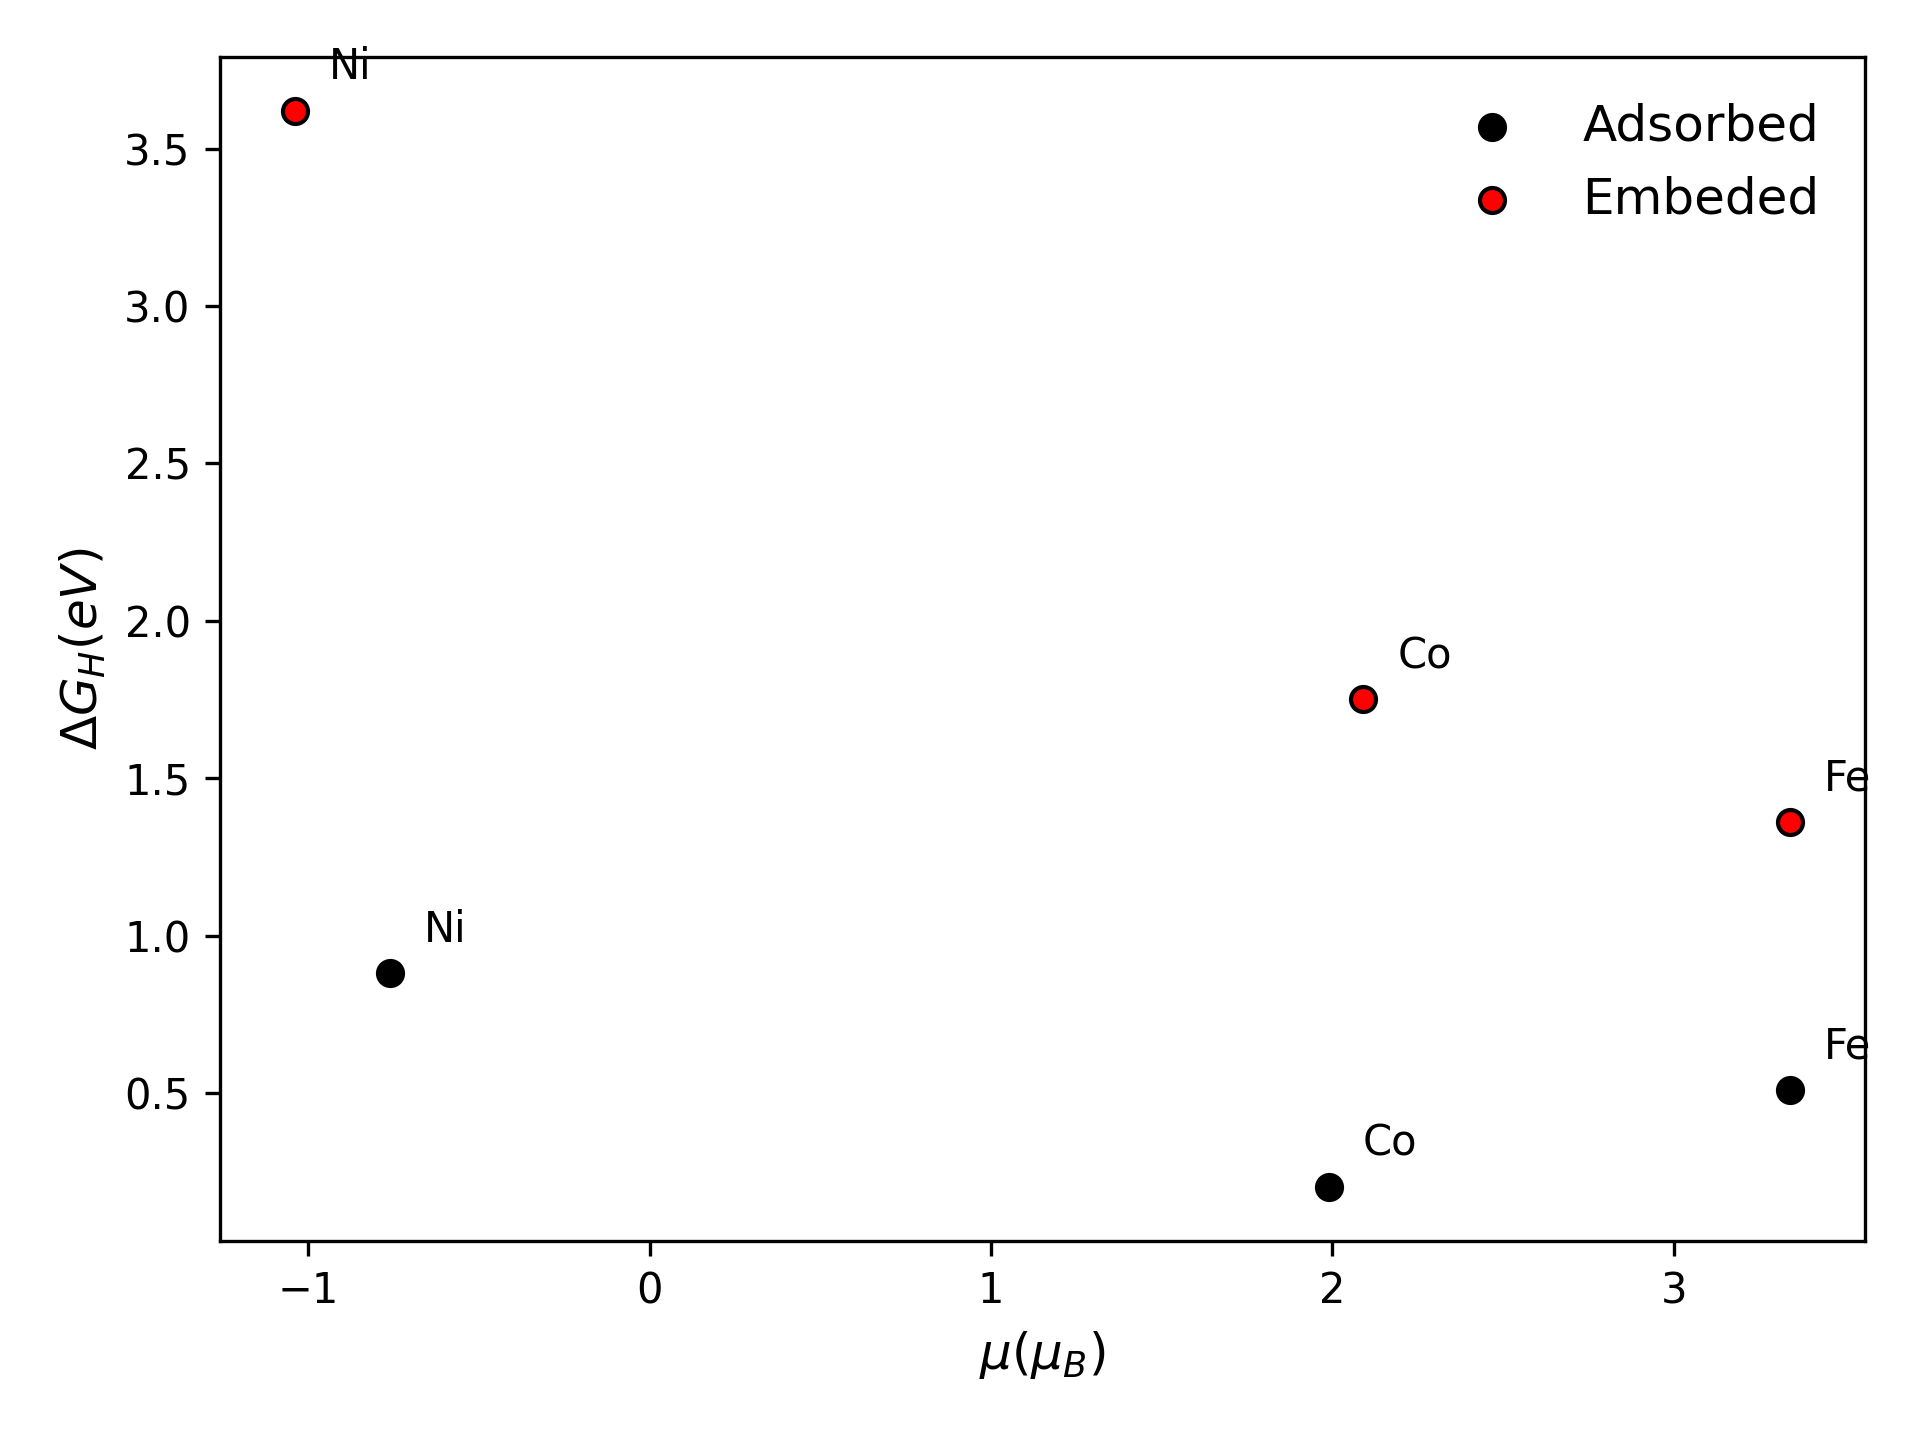
\includegraphics[width=0.8\linewidth]{figure/mu_vs_dG.png}
        \caption*{Fig. S6. Relationship between the magnetic moment ($\mu_{\mathrm{B}}$) of the transition-metal atoms and the corresponding hydrogen adsorption free energy ($\Delta G_{\mathrm{H}}$) for Co-, Fe-, and Ni-functionalized CrCl$_3$ monolayers in adsorbed and embedded configurations.}
        \label{fig:S6}
    \end{figure}



\end{suppinfo}
\end{document}